\chapter{Application requirements}
\label{chap:ch4}

\section{Android application requirements}
\label{sec:ch4sec1}

\par For our application the minimum SDK version is 23. This means that any Android device that has an Android version greater or equal to 6 (code named "Marshmallow") will be able to run our application. However there is a second requirement and that is to have NFC capabilities.

\section{Server application requirements}
\label{sec:ch4sec2}

\par Our server runs on Ktor, but there are no specified system requirements for it. However it requires an IntelliJ IDEA Ultimate as it is a proprietary plugin for Kotlin made by JetBrains. The requirements for the IDE are shown in figure \ref{fig:requirements-intelij}.

\begin{figure}
\centering
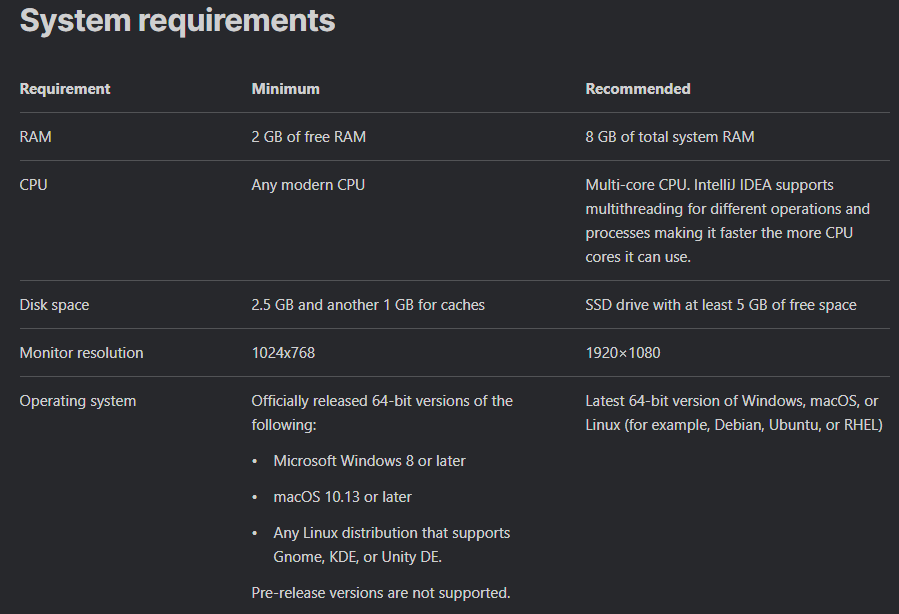
\includegraphics[width=\textwidth]{figures/system_requirements_intellij.png}
\caption{The system requirements for IntelliJ IDEA. \cite{intellijIdea}}
\label{fig:requirements-intelij}
\end{figure}

The server application also uses PostgreSQL 13.2 for its database. The requirements for this version were not made public, however we were able to find the system requirements for the previous version (12.0) so we will suppose that those stayed the same. The requirements can be seen in figure \ref{fig:requirements-postgresql}.

\begin{figure}
\centering
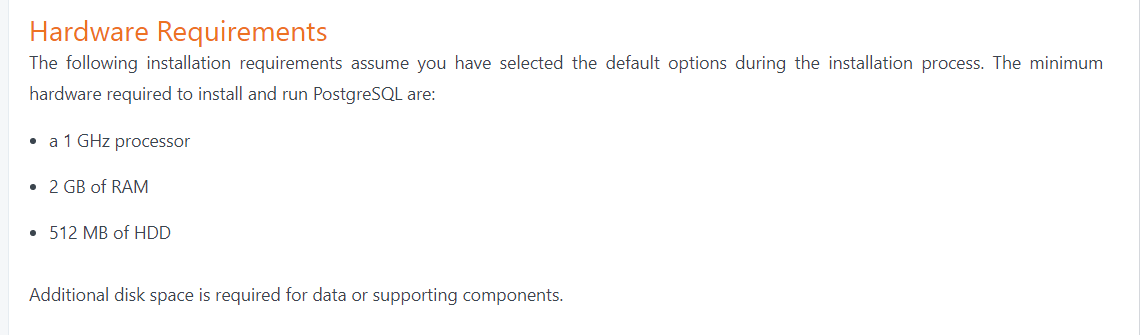
\includegraphics[width=\textwidth]{figures/postgresql_requirements.png}
\caption{The system requirements for PostgreSQL 12.0. \cite{postgresSql}}
\label{fig:requirements-postgresql}
\end{figure}